\documentclass[12pt]{article}
\usepackage{moodle}
\usepackage{graphicx}
\usepackage{xpatch}

\makeatletter
\def\graphicspath#1{\def\Ginput@path{#1}\edef\moodleimgpath{\@firstofone#1}}
%

\xpatchcmd{\moodle@includegraphics@int@int}%
{\openssl\otherspace enc -base64 -in \moodleimgpath#2.png -out #2.enc}%
{\openssl\otherspace enc -base64 -in \moodleimgpath#2.png -out #2.enc}%
{\typeout{patch ok}}%
{\typeout{patch failed}}
\makeatother

\graphicspath{{./img/}}

\begin{document}

\begin{quiz}{Newton laws}
  \begin{multi}[shuffle=true, points=1]{Newton laws - 1}
    blablabla
    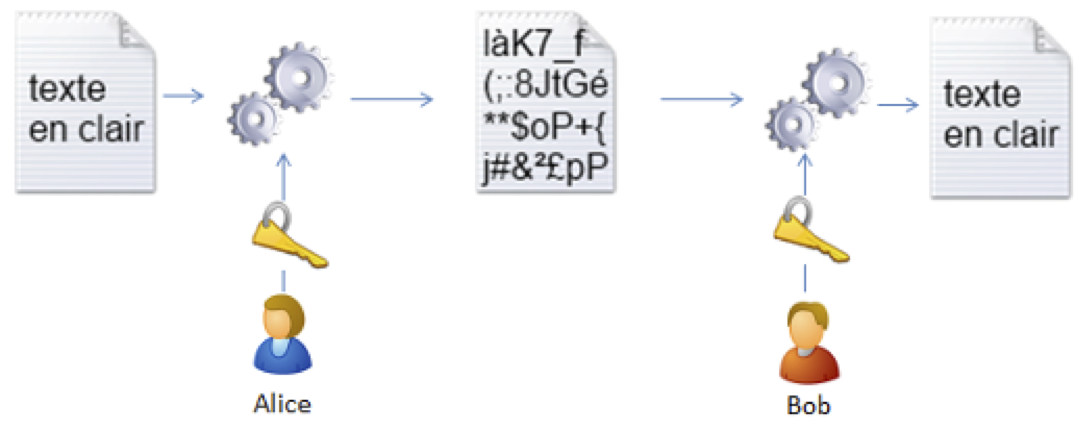
\includegraphics[width=6cm]{img/img3-20}
  \item* 1
  \item 2
\end{multi}

\end{quiz}

\end{document}
